\documentclass[tikz,border=4pt]{standalone}
% Shared look for the per-pattern diagrams. Copied from the IATEFL LTSIG talk
% (talks/doubly-personalised-language-learning/figures/llm-patterns.tex).
\usepackage{amssymb}
\usepackage{fontspec}
\setmainfont{Helvetica Neue}
\usetikzlibrary{arrows.meta,positioning,calc,fit}
\definecolor{ink}{HTML}{23373B}
\definecolor{hlc}{HTML}{C2410C}
\definecolor{okc}{HTML}{2E7D32}
\definecolor{badc}{HTML}{B91C1C}
\tikzset{
  mini/.style={rounded corners=2pt, minimum height=7mm, align=center,
               font=\small\color{ink}, fill=white, draw=ink!70, line width=0.6pt, inner sep=3pt},
  minillm/.style={mini, fill=hlc, draw=hlc, font=\small\bfseries\color{white}},
  fixed/.style={mini, fill=ink!12},                 % the fixed part of a prompt
  sarr/.style={-{Stealth[length=2mm]}, ink, line width=0.8pt},
  lbl/.style={font=\footnotesize\itshape\color{ink!75}},
  ok/.style={font=\small\bfseries\color{okc}},
  bad/.style={font=\small\bfseries\color{badc}},
}

% Prompt Amortization: one fixed preamble, paid once per batch.
% Fan-in packs many inputs into one call; fan-out asks for many outputs at once.
\begin{document}
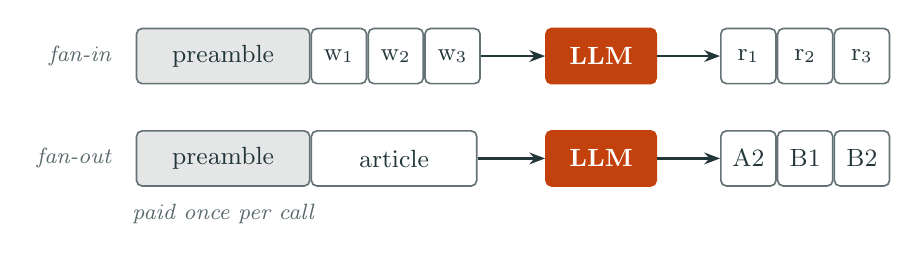
\begin{tikzpicture}[cell/.style={mini, minimum width=7mm, inner sep=1pt}]
% fan-in
\node[lbl, anchor=east] at (-0.2,0) {fan-in};
\node[fixed, minimum width=22mm] (p1) at (1.1,0) {preamble};
\node[cell, right=0pt of p1] (i1) {w\textsubscript{1}};
\node[cell, right=0pt of i1] (i2) {w\textsubscript{2}};
\node[cell, right=0pt of i2] (i3) {w\textsubscript{3}};
\node[minillm, minimum width=14mm, ] (l1) at (5.9,0) {LLM};
\node[cell, right=8mm of l1] (o1) {r\textsubscript{1}};
\node[cell, right=0pt of o1] (o2) {r\textsubscript{2}};
\node[cell, right=0pt of o2] (o3) {r\textsubscript{3}};
\draw[sarr] (i3) -- (l1); \draw[sarr] (l1) -- (o1);

% fan-out
\node[lbl, anchor=east] at (-0.2,-1.3) {fan-out};
\node[fixed, minimum width=22mm] (p2) at (1.1,-1.3) {preamble};
\node[cell, right=0pt of p2, minimum width=21mm] (a) {article};
\node[minillm, minimum width=14mm, ] (l2) at (5.9,-1.3) {LLM};
\node[cell, right=8mm of l2] (b1) {A2};
\node[cell, right=0pt of b1] (b2) {B1};
\node[cell, right=0pt of b2] (b3) {B2};
\draw[sarr] (a) -- (l2); \draw[sarr] (l2) -- (b1);

\node[lbl, below=1mm of p2] {paid once per call};
\end{tikzpicture}
\end{document}
